%%%%%%%%%%%%%%%%%%%%%%%%%%%%%%%%%%%%%%%%%
% Stylish Article
% LaTeX Template
% Version 2.1 (1/10/15)
%
% This template has been downloaded from:
% http://www.LaTeXTemplates.com
%
% Original author:
% Mathias Legrand (legrand.mathias@gmail.com) 
% With extensive modifications by:
% Vel (vel@latextemplates.com)
%
% License:
% CC BY-NC-SA 3.0 (http://creativecommons.org/licenses/by-nc-sa/3.0/)
%
%%%%%%%%%%%%%%%%%%%%%%%%%%%%%%%%%%%%%%%%%

%----------------------------------------------------------------------------------------
%	PACKAGES AND OTHER DOCUMENT CONFIGURATIONS
%----------------------------------------------------------------------------------------

\documentclass[fleqn,10pt]{SelfArx} % Document font size and equations flushed left

\usepackage[english]{babel} % Specify a different language here - english by default

\usepackage{lipsum} % Required to insert dummy text. To be removed otherwise

%----------------------------------------------------------------------------------------
%	COLUMNS
%----------------------------------------------------------------------------------------

\setlength{\columnsep}{0.55cm} % Distance between the two columns of text
\setlength{\fboxrule}{0.75pt} % Width of the border around the abstract

%----------------------------------------------------------------------------------------
%	COLORS
%----------------------------------------------------------------------------------------

\definecolor{color1}{RGB}{0,0,90} % Color of the article title and sections
\definecolor{color2}{RGB}{0,20,20} % Color of the boxes behind the abstract and headings

%----------------------------------------------------------------------------------------
%	HYPERLINKS
%----------------------------------------------------------------------------------------

\usepackage{hyperref} % Required for hyperlinks
\hypersetup{hidelinks,colorlinks,breaklinks=true,urlcolor=color2,citecolor=color1,linkcolor=color1,bookmarksopen=false,pdftitle={Title},pdfauthor={Author}}

%----------------------------------------------------------------------------------------
%	ARTICLE INFORMATION
%----------------------------------------------------------------------------------------

\JournalInfo{Data Mining B565 Fall 2016} % Journal information
\Archive{All work herein is solely ours.} % Additional notes (e.g. copyright, DOI, review/research article)

\PaperTitle{Analysis and Prediction of House Prices for the City of Ames} % Article title

\Authors{Anusha Ramamurthy(anuramam)\textsuperscript{1}, Vandana Kolli(kolliv)\textsuperscript{2}} % Authors

\affiliation{\textsuperscript{1}\textit{ Data Science, School of Informatics and Computing, Indiana University, Bloomington, IN, USA}} % Author affiliation
\affiliation{\textsuperscript{2}\textit{ Computer Science, School of Informatics and Computing, Indiana University, Bloomington, IN, USA}} % Author affiliation
\affiliation{\textbf{}} % Corresponding author

\Keywords{house --- price --- prediction --- Ames --- Iowa} % Keywords - if you don't want any simply remove all the text between the curly brackets
\newcommand{\keywordname}{Keywords} % Defines the keywords heading name

%----------------------------------------------------------------------------------------
%	ABSTRACT
%----------------------------------------------------------------------------------------

\Abstract{For decades, real estate has always been an asset most of us would like to invest on. Buying a house is never an easy decision. A number of factors influence the choice. The neighborhood, the type of architecture, the number of bedrooms so on. In this paper, we analyze 80 attributes, about 1460 houses to predict the final price of a house by applying data mining algorithms. The dataset describes the sale of individual residential properties in the City of Ames, Iowa between 2006 to 2010. We built models using linear regression, decision trees and Ada boost to predict the house prices. The results show that data mining algorithms produces high prediction accuracy in house price analysis and prediction. }

%----------------------------------------------------------------------------------------

\begin{document}
	
	
	\flushbottom % Makes all text pages the same height
	
	\maketitle % Print the title and abstract box
	
	\tableofcontents % Print the contents section
	
	\thispagestyle{empty} % Removes page numbering from the first page
	
	%----------------------------------------------------------------------------------------
	%	ARTICLE CONTENTS
	%----------------------------------------------------------------------------------------
	\section{Introduction} % The \section*{} command stops section numbering
	\subsection{Problems in House Price Prediction}
	Real estate properties have always been a safe option of investment. It is an investment that does not decline in value rapidly. The  growing real estate industry has become an important part of national economy. Problems such as rapid increase in house prices, high vacancy ratio require the Government to institute industrial policies to help bridge the gap. With the increase in data, analysts can apply tools to predict house prices to help consumers. A lot of housing data is available today, with different features like Lot Area, Street, neighborhood etc. The idea is to find an efficient data analysis methodology to transform these datasets into significant sources of knowledge and information\cite{irb}.\\
	
	The data comprises of the multiple features of the house which can be considered by potential buyers. However it is impossible to provide an automated comparison on all the features as they are diverse. This diversity makes it challenging to predict the correct market price. Feature Extraction is one of the biggest challenges faced with data having a large feature set.
	
	\subsection{Data Minning on House Price prediction}
	Data mining is the process of understanding useful and structural patterns in data, thus referring to the overall procedure of information discovery from data. These data specific discoveries became popular in the domain of machine learning and artificial intelligence. Some of the most popular machine learning algorithms include - decision trees, linear regression, logistic regression, neural networks, random forests and so on. Each algorithm suits some problems better than others. Data mining techniques are used to extract knowledge from data using a different of methods that are broadly divided in two groups: classification and regression. Classification learns to map, or classify, an item into one of the several predefined classes while regressions maps the item to a continuous numerical prediction.\\
	
	Data mining draws inferences from data to understand the patterns of correlation among data values and to predict the future data values. By calculating the differences between the actual and predicted price as an error, we compare the results and accuracy of the predicated prices by the use of Decision Trees and Ada Boost algorithms. 
	
	\subsection{Interests and Motivation}
	The world today is rapidly changing. People travel miles without a kin or friend, to newer unseen places. It is hard to find some one to consult with before buying a house in a new town. These changing times demand an undisputed, unparalleled authority to help the general public, get an unbiased prediction on the price of a house. Tax payers need help to evaluate their yearly tax projections. It is also an interesting challenge for data miners and computer scientists. Identifying the features based on demographics, current market trends, patterns in personal and housing loans, every little factor influences the real estate market. Data mining algorithms and analysis feed on such factors to help make informed data driven decisions. 

	
	%------------------------------------------------
	
	\section{Background}
	
	\begin{figure*}[ht]\centering % Using \begin{figure*} makes the figure take up the entire width of the page
		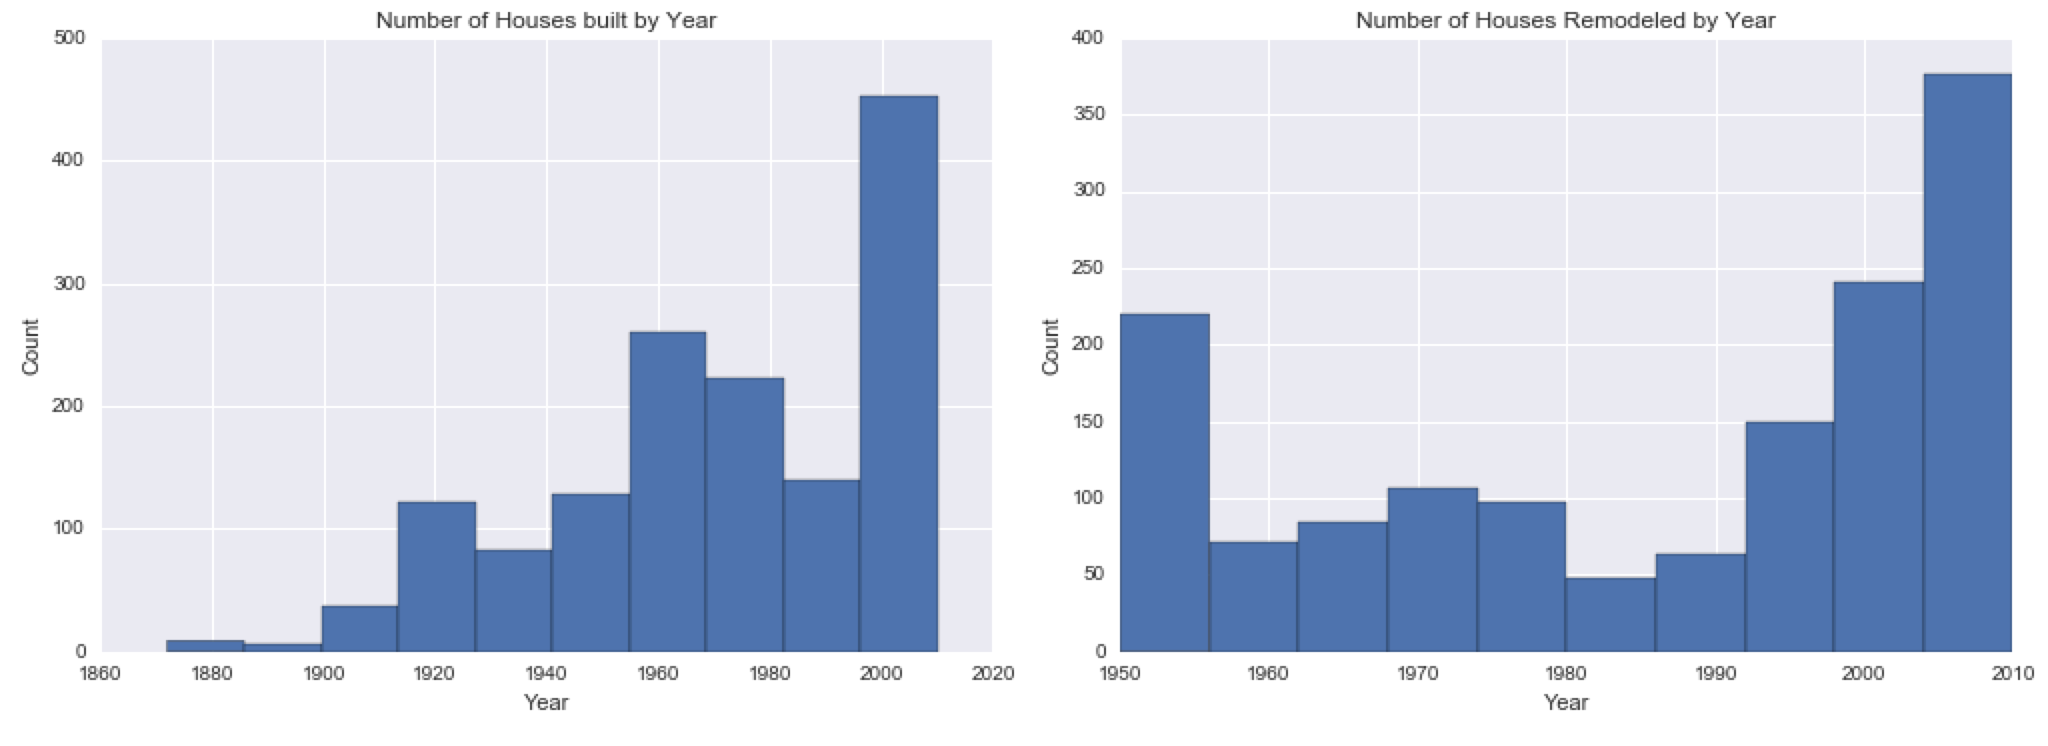
\includegraphics[width=\linewidth]{year}
		\caption{Count of Houses Built and Remodeled}
		\label{fig:year}
	\end{figure*}
	\begin{figure*}[ht]\centering % Using \begin{figure*} makes the figure take up the entire width of the page
		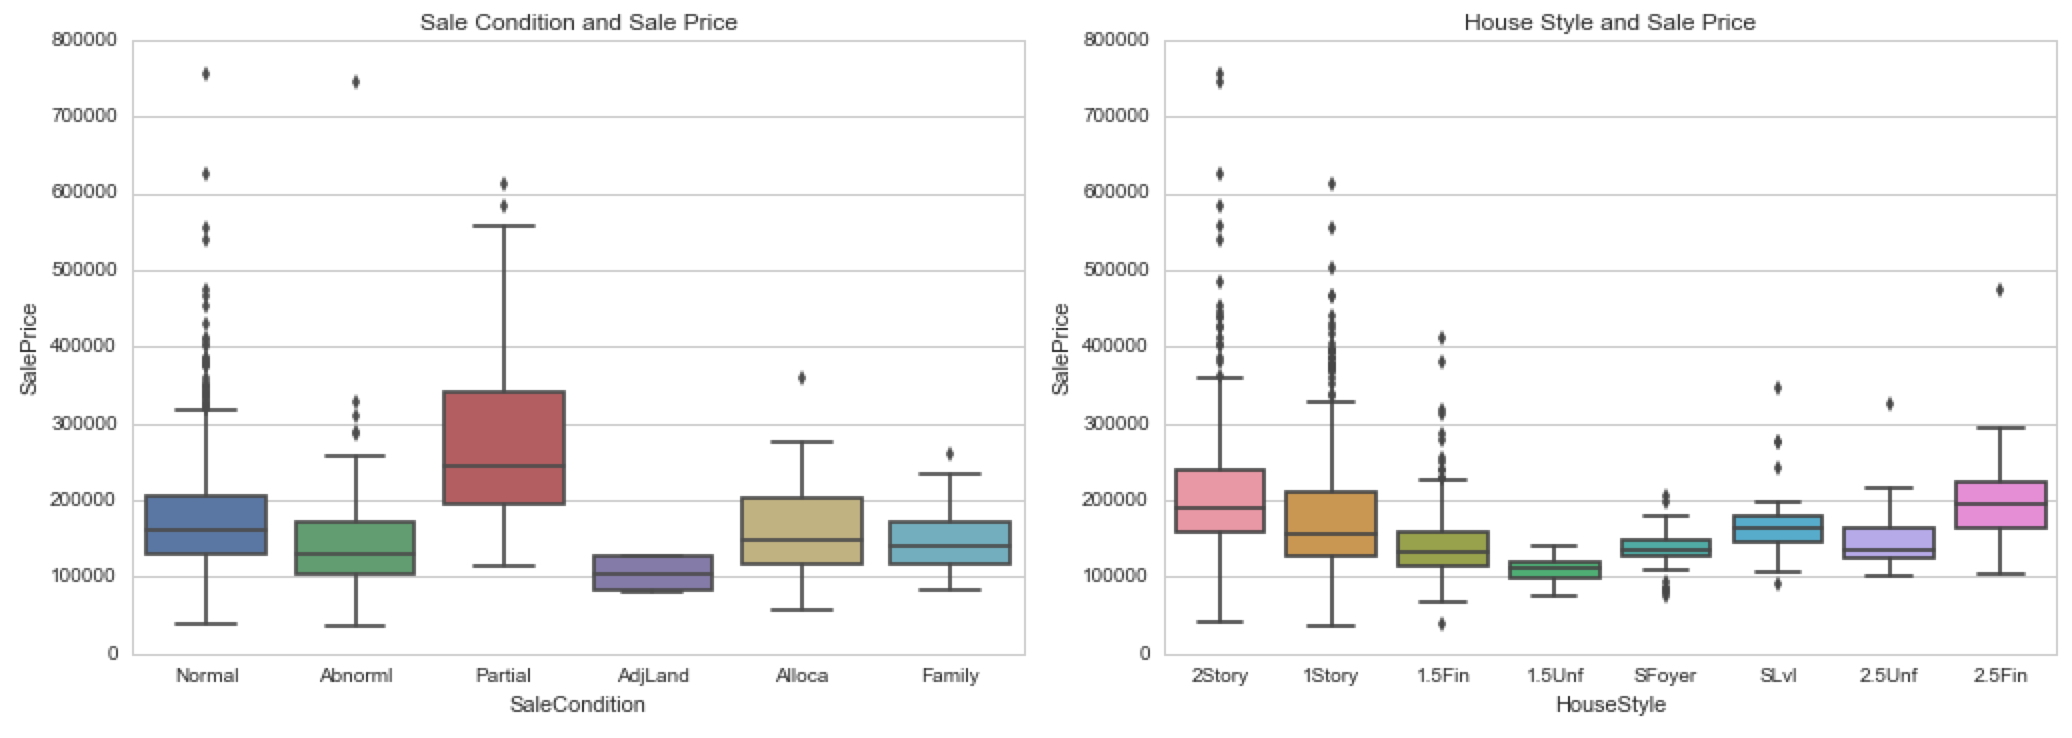
\includegraphics[width=\linewidth]{SalePrice}
		\caption{Distribution of Sale Price}
		\label{fig:SalePrice}
	\end{figure*}

	Data is of various types. Some describe a value that is individual and distinct. These are termed as Discrete Data. Some can take on an infinite number of values and are termed Continuous Data types.  Some Data values fall under different categories and are discrete, like the color one likes. These types are termed as Nominal Data. Then there are data types that preserve the ordering where the actual value doesn't matter except to signify the rank. These are called Ordinal data types. \\
	
	Attributes are properties that provide information about an item. Observations are a set of attributes that talk about a single item under discussion. Null values are attributes with no value specified.\\
	
	In this paper we used machine learning algorithms like linear regression, decision trees and Ada Boost to predict the house prices. Machine learning techniques can be divided into supervised and unsupervised. Our analysis takes into consideration the provided target variables in making predictions, thus it is supervised. In this section we will discuss about these techniques in detail.
	
	\subsection{Linear Regression}
	
	A Regression Model defines three types of regression models: linear, polynomial, and logistic regression. Linear regression, the most widely used of all statistical techniques, allows to summarize and study relations between two continuous variables\cite{stat}. It attempts to model the relationship between these two variables by fitting a linear equation to observed data. \\
	
	Let $Y$ be the target value which we need to predict.\\
	
	Let $X$ be the independent variables from which target is predicted, then the linear regression line has an equation of the form:\\
	\footnote{where $a$ and $b$ are constants.}\centerline{\[ $Y = a + bX$\]}	
	
	
	Most common method to fit a regression line is the method of least squares which calculates the best fitting line for observed data by minimizing the sum of squares of the vertical deviations from each data point to the line. 
	
	\subsection{Decision Trees}
	A decision tree builds regression or classification models in the form of a tree structure. The tree includes root node, branches and leaf nodes. Each internal node denotes a test on an attribute, each branch denotes the outcome of a test and each leaf node holds a class label. Decision trees can handle both categorical and numerical data. \\
	Different algorithms and impurity measures are used for building a Decision Tree. In our analysis we have used CART (Classification and Regression Tree) algorithm. In our paper since we are dealing with prediction of a continuous  variable(price), the decision tree is called regression tree.\\
	
	\textbf{Gini Index}\\
	It measures the inequality among values of a frequency distribution. Gini index of 0 means perfect equality(where all values are same) and Gini index of 1 means maximum inequality among values. The impurity(or purity) measure used in building decision tree in CART is called GINI index.
	\[Gini Index = 1 - \sum_{j}p_j^2 \]
	
	\subsection{AdaBoost Algorithm}
	AdaBoost algorithm was the first practical demonstration of boosting by Freund and Schapire\cite{adaboost}. Boosting in general is a machine learning approach that demonstrates the idea that a collection of week predictors can be combined to come up with a strong predictor. 
	
	%------------------------------------------------
	
	\section{Methods and Data Analysis}
	
	\subsection{Data Description}
	The dataset consisted of information about 2919 houses in the City of Ames, Iowa, United States of America. These houses were split into two sets, one  with information about 1460 houses, each has 81 attributes, 79 of them describe various aspects and quality of the house, two others being the ID, identification number for each house and the other is an attribute we wish to predict, the Sale Price of the house. Among the 79, we found 23 attributes to be nominal, 23 to be ordinal, 14 were discrete and 19 continuous set of values \cite{dataset}.\\
	
	\begin{table}[hbt]
		\caption{Table of Attribute Types}
		\centering
		\begin{tabular}{llr}
			\cmidrule(r){1-2}
			Attribute Type & Count \\
			\midrule
			Nominal & 23 \\
			Ordinal & 23 \\
			Discrete & 14 \\
			Continous & 19
		\end{tabular}
		\label{tab:label}
	\end{table}
	
	All the continuous variables are the dimensions measured in square feet, for example the size of the lot, the basement area, the size of the living area and so on. The 14 discrete variables are the count of the various commodities present in the house, for example the count of the bedrooms, bathrooms and so on. The 46 categorical variables describe aspects like the quality of the house, fireplace pool and so on, as well as information about the neighborhood the house belongs to. Hence we couldn't eliminate missing values as there would be no row available.\\
	
	\subsection{Exploratory Analysis}
	We begin our analysis by checking for duplicates, a check of Id values showed 1460 unique observations. We found that among the 81 attributes, 19 of them had missing values. An initial exploratory analysis of the 62 attributes that had no missing values revealed some interesting insights. \\
	
	A thousand four hundred and sixty houses were sold in just four years. The year 2009 appears to have seen the highest number of sales with 338 houses sold. Around 551 of the house's appear to have been built between 1999 and 2010, while 909 of the houses that were sold between 2006 and 2010,  were built between 1870 and 1989. Around 178 of these houses were remodeled in the year 1950, 20 of these were built in the year 1920. Clearly the year a house was built seems to be a factor in the sale of a house, but only further investigations can say if it was an advantage or not. Does the age of house make it more attractive to a buyer? It appears hard to say. From the graphs, most of the houses appear to have been remodeled during 1950-1955 and 2000-2010. \\
	
	It also appears that amongst most forms of Sale, Normal conditions of the sale appear to have fetched the highest price. But, houses that were not complete when last assessed also seem to fetch a higher price(Partial Condition). In fact looking at the distribution it appears that these fetched a broader range of prices than most other form of Sale Conditions. It also appears that Two story houses fetched the highest price as well as having Two and one-half story and One story houses fetched the next best prices. In both graphs we see houses that fetched a very high price, these may be possible outliers. 
	
	\subsection{Missing Values}
	A large part of analysis depends on the amount of data we have. A large volume of data allows our  data mining algorithms to train better and eventually reduce the margin of error. With the current data set we found 19 attributes containing missing values. Every row of our observations had at least one attribute with a missing value. 
	
	\begin{table}[hbt]
		\caption{Table of Missing Values}
		\centering
		\begin{tabular}{llr}
			\cmidrule(r){1-2}
			Attribute Name &  Type & Missing \\
			\midrule
			Electrical & Nominal & 1 \\
			MasVnrType & Nominal & 8 \\
			MasVnrArea & Continous & 8 \\
			BsmtQual & Nominal & 37 \\
			BsmtCond & Nominal & 37 \\
			BsmtExposure & Nominal & 38 \\
			BsmtFinType1 & Nominal & 37 \\
			BsmtFinType2 & Nominal & 38 \\
			GarageType & Nominal & 81 \\
			GarageYrBlt & Continuous & 81 \\ 
			GarageFinish & Nominal & 81 \\
			GarageQual & Nominal & 81 \\
			GarageCond & Nominal & 81 \\
			LotFrontage & Continuous & 259 \\
			FireplaceQu & Nominal & 690 \\
			Fence & Nominal & 1179 \\
			Alley & Nominal & 1369 \\
			MiscFeature & Nominal & 1406 \\
			PoolQC & Nominal & 1453 \\	
		\end{tabular}
		\label{tab:label}
	\end{table}

	\subsection{Replacing Missing Values}
	Looking at each of the missing attributes we had to find a way to fill them without loss of existing relationships and natural distribution of the data. Some of the existing methods to replace missing values is by filling them with the mean , median or the mode. Since 16 of our missing values are Nominal data types, mean and median are meaningless. If we choose to replace them by the mode blindly, we might make our data skewed. Hence we decided to look at each attribute of the house, before we fill the missing values. \\
	
	For the Electrical Attribute, it could take the four possible values. We found that 'FuseA' appeared to be the most common type of electrical type across homes of in the 'Timber' Neighborhood and replaced our missing value with the same. Attributes Masonry veneer type and Masonry veneer area appeared to be linked. For values of Masonry veneer type as 'None', the Masonry veneer area always had 0.0 square feet as the value. For those observations where Masonry veneer area alone was missing, the Masonry veneer type was also missing. Hence we filled Masonry veneer type as  'None' and Masonry veneer area with values '0.0'.\\ 
	
	Attributes 'BsmtQual', 'BsmtCond',    'BsmtExposure',\\
	'BsmtFinType1', 'BsmtFinType2' also appear to be related as they describe properties of the basement area of the house. We found that these attributes that were missing for the observations appeared to be houses with no basements. On analysis we found that the BsmtFinSF1, BsmtUnfSF, TotalBsmtSF which were values about the dimensions of the basement were all zero. Hence we filled each of the missing values with 'NA', which conveys the information that no basement is present. 
	
	Attributes 'GarageType','GarageFinish, 'GarageQual',\\'GarageCond', 'GarageYrBlt' give description about the garage of the house. These values appear to be missing for houses that had no garage. Hence we filled each of these values with NA, except the attribute 'GarageYrBlt' which we felt was not as informative if there is no garage in the first place. For most houses the 'GarageYrBlt' appears to be the year the house was built. Hence we choose to remove this attribute all together. For the attribute 'FireplaceQu' we have no other correlated attribute that could give us an intuition on how to fill its missing values. We decided to assume that the missing values signify a house without a fire place, as most houses in Ames appear to have Central heating and filled it with 'NA'. We did the same for attributes 'PoolQC' and 'MiscFeature' as they appear to be for housings without a pool or any other miscellaneous feature like elevators. For the attribute 'Fence', we assumed that most houses would have the bare minimum fencing and replaced it with 'MnWw' which stands for minimum wood or wire fencing. For the attribute 'Alley' we choose to fill this attribute with 'NA' after a study of the document on Housing Information, on the City of Ames website which stated that attribute 'LotFrontage' and 'Alley' need not have a minimum value\cite{ames}.
	\begin{figure*}[ht]\centering % Using \begin{figure*} makes the figure take up the entire width of the page
		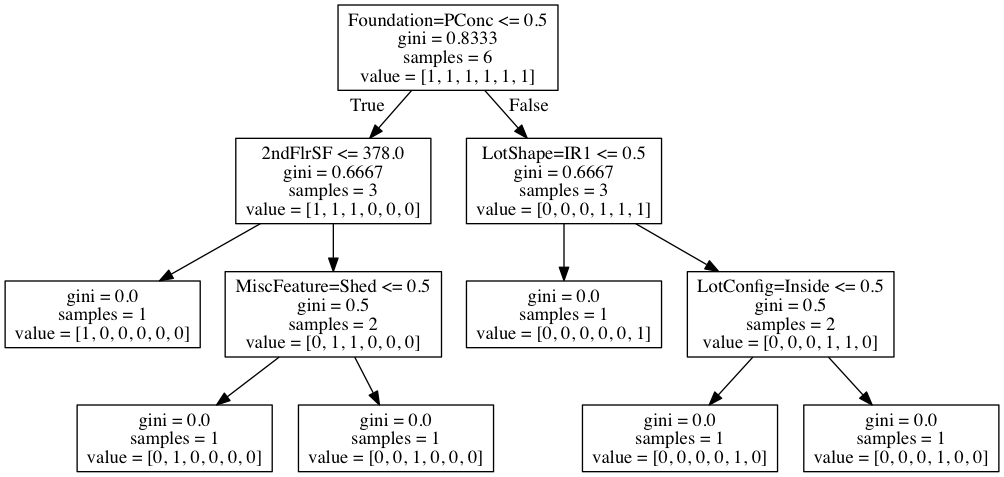
\includegraphics[width=\linewidth]{tree_diagram_10samples}
		\caption{Decision Tree for 10 observations}
		\label{fig:tree_diagram_10samples}
	\end{figure*}
	\begin{figure*}[ht]\centering % Using \begin{figure*} makes the figure take up the entire width of the page
		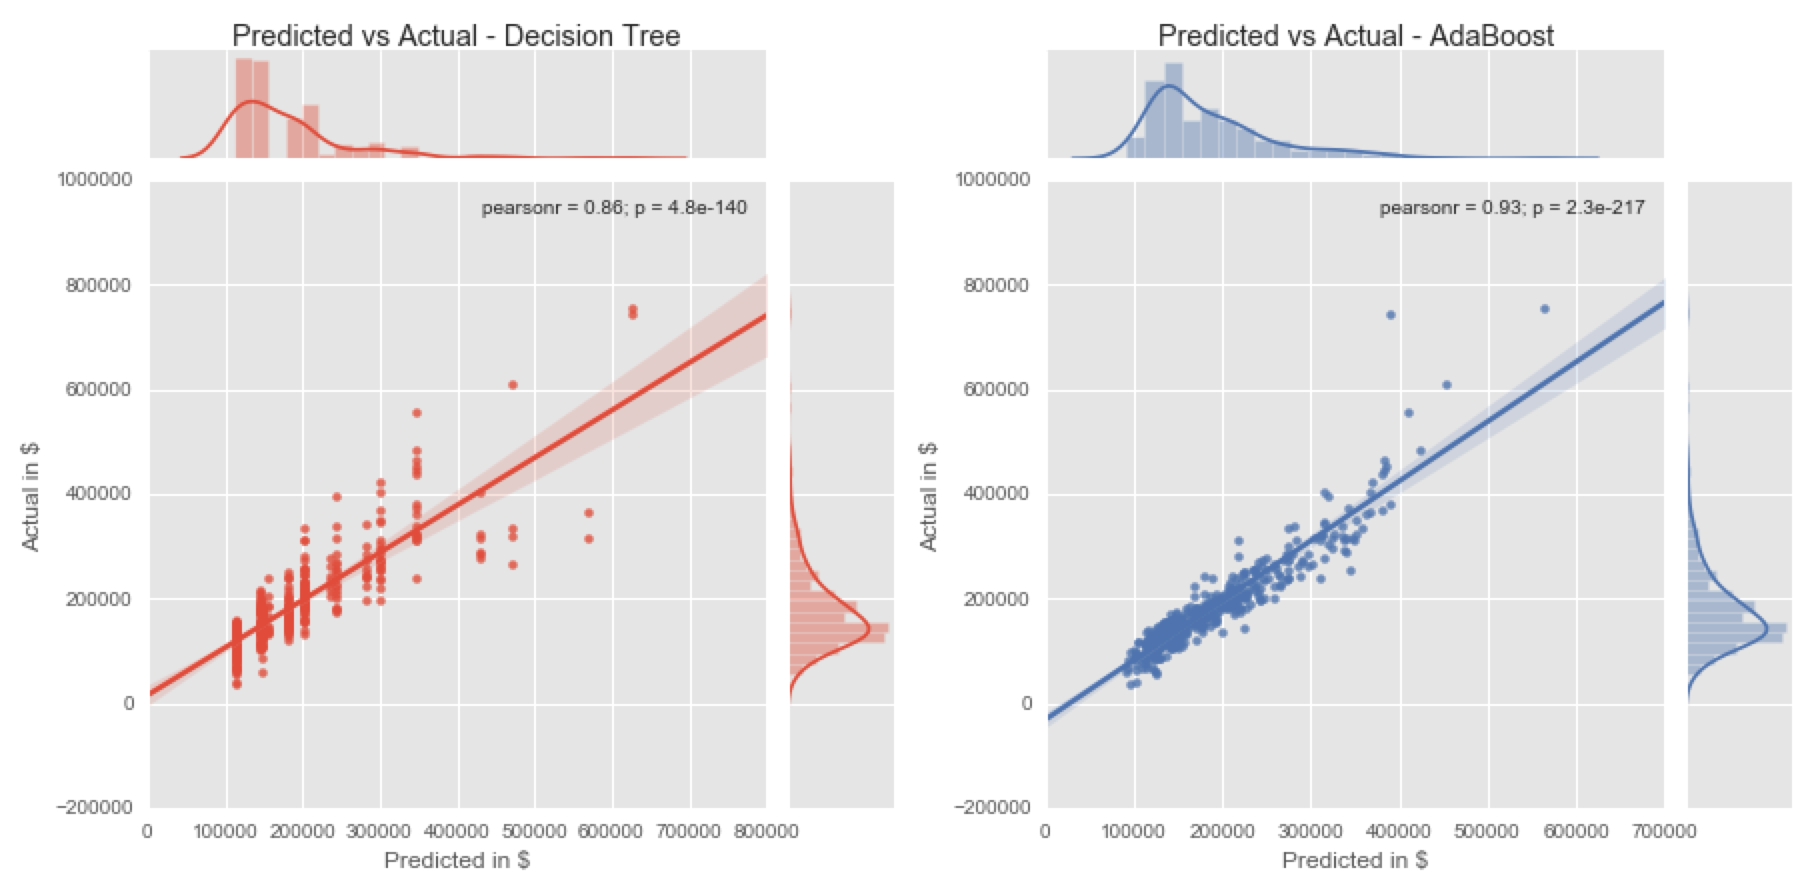
\includegraphics[width=\linewidth]{results}
		\caption{Results}
		\label{results}
	\end{figure*}
	
	\section{Problem}
	We now have a complete dataset, with 78 attributes that could help us in determining the price of the house. We choose to first build a linear model to predict the Sale Price. This was motivated by the paper on this dataset described in \cite{dataset}. This problem was and is assumed to be a best solved by regression models. It is intuitive to think that each extra bedroom would cost $x$ amount of cash, so we assume that the independent components of the house linearly influence the price of the house. For example \\
	$Cost_{(house_{(i)})} \\
	= (Number_{(bedrooms)} * Area_{(bedroom)}+Number_{(bathrooms)}\\*Area_{(bathroom)}+Number_{(kitchens)}*Area_{(kitchen)})* Cost_{(persqfeet)}$\\
	
	However, most of us while looking for a house, either like one aspect of the house more than anything else. So for some person X, the best think is a porch, and the price X would pay for it is not a tangible value. We have no way of quantifying a likable attribute. Hence in our opinion, a linear equation for such a problem has its own caveats. What we needed was an algorithm that will look at all the existing training samples and learn the distribution without making prior opinions about the parametric nature of the problem.\\
	
	Hence we choose to next apply a non parametric algorithm. Decision trees are popular algorithms that create branching by asking yes or no questions. CART or Classification and Regression Trees are extensively used in Predictive Modeling. A regression tree partitions each observation such that those with same values are grouped together. Hence it maintains the natural grouping of the data. A tree produced by the algorithm for small set of 10 observations is included. \\
	
	A Decision Tree can over fit and not generalize well. Hence it fails to perform well on new observations. One method to over come the bias and variation is by using Boosting \cite{dt}. A set of weak decision trees are combined with adjusted weights\cite{ada}. Adaptive boosting or AdaBoost implementation was hence used to generate better results. 
	
	
	\section{Experiments}
	 \begin{table}[hbt]
	 	\caption{Table of Implementation Specifications}
	 	\centering
	 	\begin{tabular}{llr}
	 		\cmidrule(r){1-2}
	 		Name &  Type \\
	 		\midrule
	 		Operating System & MAC Sierra \\
	 		RAM Size & 16 GB\\
	 		Programming Language & Python \\
	 		Version & 2.7\\
	 		Editor & Ipython Notebook \\
	 		Libraries & pandas, scikit-learn, NumPy\\
	 		& matplotlib,pydotplus,graphviz 
	 	\end{tabular}
	 	\label{tab:label}
	 \end{table}
	 The data was present as a competition in the Kaggle website\cite{kaggle}. A detailed description of the attributes is also present. The data set is split into two files, one with the Sale Price given, the other without. We used the data file with the Sale Price present to implement and test our hypothesis. We began by doing some initials checks on the data set, like the size of the data set, the attributes. We then moved to the cleaning and preprocessing of the dataset. This involved the process of finding and replacing the missing values. \\
	 
	 All of our implementation was using Python programming. For most regression algorithms, the data has to be of Real values, namely continuous data types. Hence we had to use a method of changing our nominal data types to real valued numbers\cite{dict}. \\
	 
	 We split our Data set into 70-30 ratio. 70\% of our data is split to train the algorithm and 30\% is used in testing. We applied Linear Regression, Decision Tree and AdaBoost for Decision Tree Regressors We also applied K-fold Cross Validation methods for each algorithm\cite{kfold}.
	
	
	\section{Results}
	We trained our algorithms with 78 attributes, to predict the House Prices. Linear regression yielded extremely poor results. We then applied Decision Tree Regressor For the 70 training,30 test split it yielded a score 61\%. On K-fold cross validation with $k=10$ Decision trees gave better score of 76\%.\\
	
	We then applied AdaBoost for Decision Tree Regressor For the 70 training,30 test split it yielded a score 85\%. On K-fold cross validation with $k=10$ AdaBoost gave an average score of 85\%.\\
	
	\begin{table}[hbt]
		\caption{Table of Results} \centering \begin{tabular}{llr} \toprule \multicolumn{2}{c}{70\%-30\% Train Test Split} \\ \cmidrule(r){1-2} Approach & Accuracy\\ \midrule Decision Tree & 61\% \\ 
			AdaBoost Algorithm & 85\% \\ \bottomrule \end{tabular} 
		\label{tab:label} 
	\end{table}
	
	\begin{table}[hbt]
		\caption{Table of Results} \centering \begin{tabular}{llr} \toprule \multicolumn{2}{c}{K-fold Cross Validation} \\ \cmidrule(r){1-2} Approach & Accuracy\\ \midrule Decision Tree & 75\% \\ 
				AdaBoost Algorithm & 85\% \\ \bottomrule \end{tabular} 
		\label{tab:label} 
	\end{table}
	
	From the graphs, we do se several outliers that appear to be never accurately predicted by either of the algorithms. It does appear that Decision Tree comes very close to predicted the Sale Prices, but never quite gets there. The predicted and actual prices appear to be more closer in the case of Adaboost. The Pearson Coefficient Ratio for Decision tree for Actual and Predicted values was around 0.86, while for Adaboost it was 0.93. 
	
	 
	\section{Summary conclusion}
	The results from Linear regression were disappointing, but in a way it makes sense. There are a number of features that contribute towards making the decision to buy a home and they may not all be linearly correlated. While decision trees were able to learn better, we would like to explore other algorithms and approaches to get a much better accuracy of Sale prices.
	\section{Future Work}
	In future, we would like to explore a different approach to filling the missing values to examine if the overall accuracy of predictions increase. We  would also like to work with Random forests and Lasso Regression. We would like to explore PCA and other dimensionality reduction techniques. Another idea is combining this dataset with the Boston Housing Prices Dataset to analyze if Housing Sales follow similar or different patterns across cities.
	
	%------------------------------------------------
	\phantomsection
	\section*{Acknowledgments} % The \section*{} command stops section numbering
	
	\addcontentsline{toc}{section}{Acknowledgments} % Adds this section to the table of contents
	We would like to thank Prof. Mehmet Dalkilic for giving us the opportunity and resources to work on this project. We would also like to thank Hasan Kurban and all other AIs for their help.
	
	%----------------------------------------------------------------------------------------
	%	REFERENCE LIST
	%----------------------------------------------------------------------------------------
	\phantomsection
	\bibliographystyle{unsrt}
	\bibliography{/Users/aramamurthy/Downloads/Github/Kaggle-HPAR/references.bib}
	%----------------------------------------------------------------------------------------
	
\end{document}